\documentclass{article}
\usepackage{amsmath, tikz, tcolorbox, array, multicol, sfmath, enumerate, pgfplots}
\renewcommand{\familydefault}{\sfdefault}
\pgfplotsset{compat=newest}
\usepgfplotslibrary{fillbetween}
\usetikzlibrary{arrows.meta}
\everymath{\displaystyle}
\tikzset{>=stealth}
\usepackage[top = 0.25in, bottom = 0.25in, left = 1.25in, right = 1.25in]{geometry}
\pagestyle{empty}
\raggedright

\newcounter{example}[section]
\newenvironment{example}[1][]{\refstepcounter{example}\par\medskip
   {\color{red}\textbf{Example~\theexample. #1}}}{\medskip}
\newcommand{\dx}{\, \mathrm{d}x}

\begin{document}

\section*{Area and the Definite Integral}

\begin{tcolorbox}[colframe=orange!70!white, coltitle=black, title=\textbf{Summary}]
\begin{enumerate}
    \item 
\end{enumerate}
\end{tcolorbox}
\vspace{1in}

Suppose we have a function that lies entirely above the $x$-axis. \newline\\

What would the area of the function that is above the $x$-axis be between the $x$-coordinates of $a$ and $b$ below?
\newline\\

\begin{center}
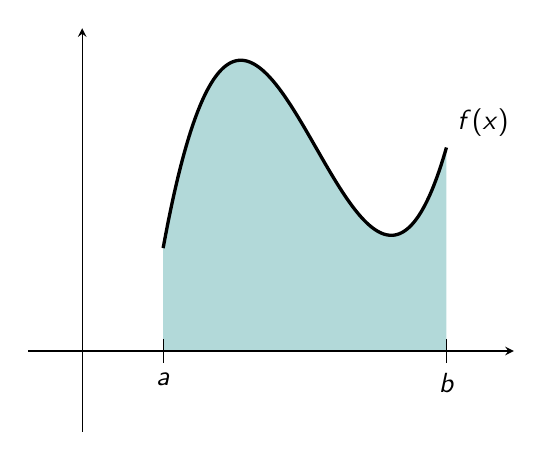
\begin{tikzpicture}[scale=0.9]
\begin{axis}
[axis lines = middle, xmin = -1, xmax = 8, ymin = -1, ymax = 4, ticks = none]
\addplot [domain = 1.5:6.75, samples=200, very thick, name path = f] {
0.2*(x-6)^3 + (x-6)^2 + 0.5*(x-6) + 1.5
} node [above right] {$f(x)$};
\path[name path=axis] (axis cs:1.5,0.015) -- (axis cs:6.75,0.015);
\addplot [
        color=teal!30,
        fill=teal!30
    ]
    fill between[
        of=f and axis, soft clip={domain=1.5:6.75}
    ];
\draw (axis cs: 1.5,0.15) -- (axis cs: 1.5,-0.15) node [below] {$a$};
\draw (axis cs: 6.75,0.15) -- (axis cs: 6.75,-0.15) node [below] {$b$};
\end{axis}
\end{tikzpicture}
\end{center}
\vspace{1in}

Or, perhaps even more importantly, \emph{how would we go about doing this?}

\newpage 

One of the most common ways to find the area under a curve is to \newline\\
\begin{center}
\fbox{use rectangles of equal width and calculate the area of each rectangle.} 
\end{center}
\vspace{1in}

We will work this out in the first example.
\vspace{0.75in}

\begin{example}
Find the area under the curve $f(x) = x^2$ , above the $x$-axis, and between $x = 1$ and $x = 5$ as follows:
\begin{enumerate}[(a)]
    \item Using 4 rectangles of equal width \newline\\
\vspace{0.25in}
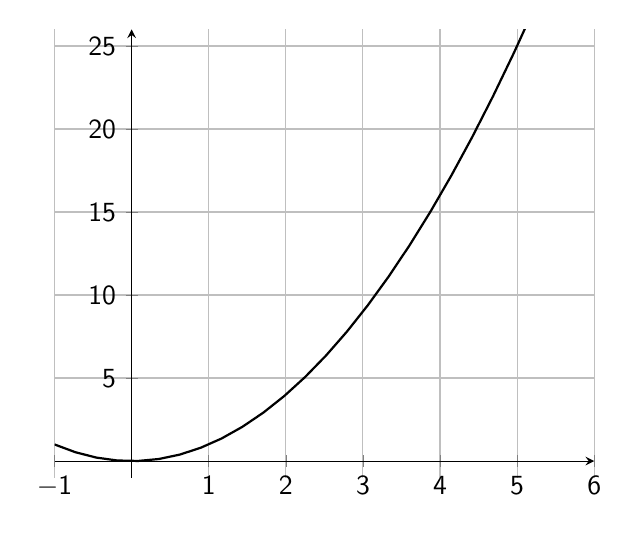
\begin{tikzpicture}
\begin{axis}
[axis lines = middle, xmin = -1, xmax = 6, ymin = -1, ymax = 26, grid]
\addplot [thick, domain=-1:5.5] plot {x^2};
\end{axis}
\end{tikzpicture}
\newpage 
    \item Using 8 rectangles of equal width \newline\\
\vspace{0.25in}
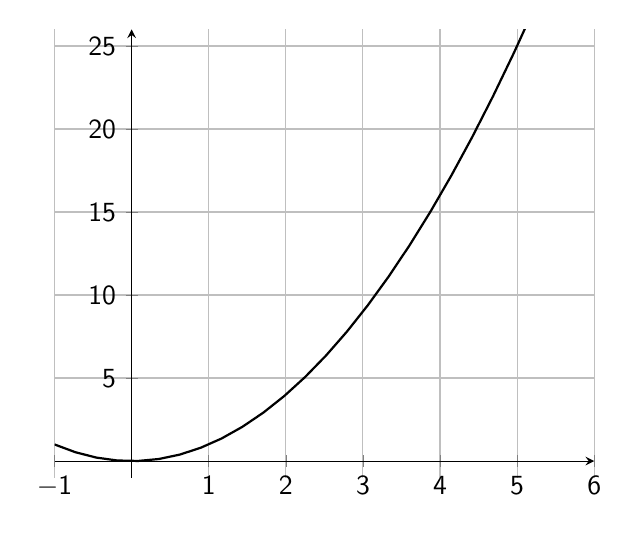
\begin{tikzpicture}
\begin{axis}
[axis lines = middle, xmin = -1, xmax = 6, ymin = -1, ymax = 26, grid]
\addplot [thick, domain=-1:5.5] plot {x^2};
\end{axis}
\end{tikzpicture}
\end{enumerate}
\end{example}
\vspace{1.25in} 

\subsection*{Using the Right Endpoints}

In the previous example, we approximated the area under the curve $f(x) = x^2$ from $x = 1$ to $x = 5$ by using rectangles. \newline\\

The heights of the rectangles were determined by $f(1)$, $f(2)$, $f(3)$, and $f(4)$. \newline\\

These were the {\color{blue}\textbf{left endpoints}} of the rectangles. However, we can also use the right endpoints.
\vfill 

\begin{example}
Using right endpoints, find the area under the curve $f(x) = x^2$ , above the $x$-axis, and between $x = 1$ and $x = 5$ as follows:
\begin{enumerate}[(a)]
    \item Using 4 rectangles of equal width \newline\\
\vspace{0.25in}
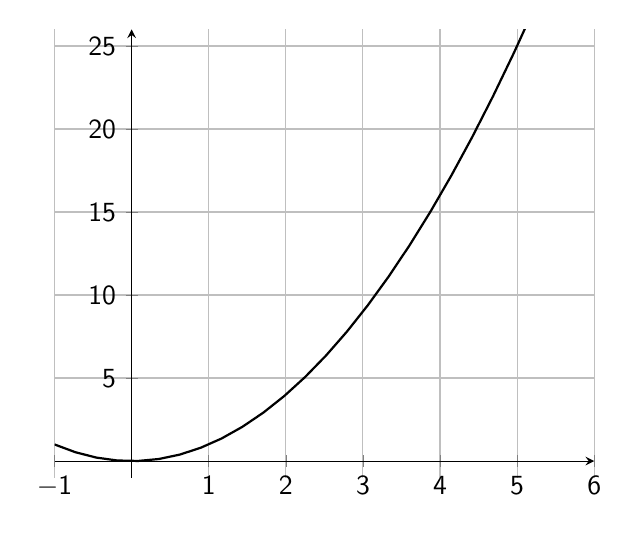
\begin{tikzpicture}
\begin{axis}
[axis lines = middle, xmin = -1, xmax = 6, ymin = -1, ymax = 26, grid]
\addplot [thick, domain=-1:5.5] plot {x^2};
\end{axis}
\end{tikzpicture}
\newpage 
    \item Using 8 rectangles of equal width \newline\\
\vspace{0.25in}
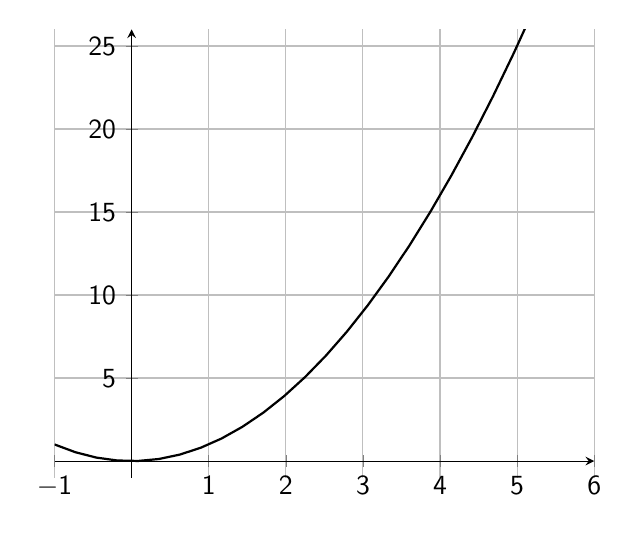
\begin{tikzpicture}
\begin{axis}
[axis lines = middle, xmin = -1, xmax = 6, ymin = -1, ymax = 26, grid]
\addplot [thick, domain=-1:5.5] plot {x^2};
\end{axis}
\end{tikzpicture}
\end{enumerate}
\end{example}
\vspace{1.25in} 

You can use any point on the width of each rectangle. \newline\\

Most of the time it will be the left or right endpoint, or the center of each rectangle.
\vspace{1.5in}

\subsection*{The Definite Integral}

As the number of rectangles on a closed interval $[a,b]$ increases indefinitely, the width of each rectangle becomes smaller and smaller. \newline\\

This will give us better and better approximations to the area under the curve. \newline\\

\begin{align*}
    \text{Area under curve} &= \text{Add up: } \left(\text{each rectangle height} \times \text{each rectangle width}\right) \\
    &= \text{Add up: } f\left(\text{each $x$ value}\right) \times \text{change in $x$ value} \\
    &= \text{Add up: } f(x) \times \text{very small change in $x$ value} \\
    &= \int_{a}^{b} f(x) \, \dx 
\end{align*}

\begin{example}
Write the definite integral to represent the shaded area of the following:
\begin{center}
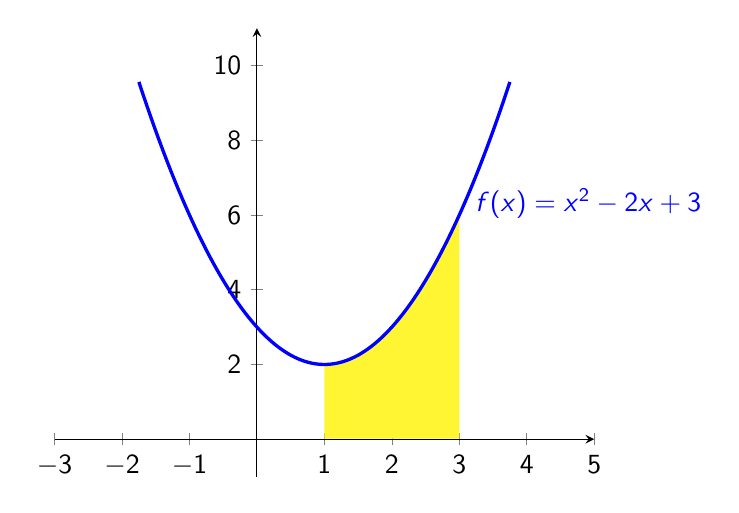
\begin{tikzpicture}
\begin{axis}
[axis lines = middle, xmin = -3, xmax = 5, xtick = {-3,-2,...,5}, ymin = -1, ymax = 11, clip=false]
\addplot [domain = -1.75:3.75, samples=200, blue, very thick, name path = f] {
x^2-2*x+3
} node [right, pos=0.8] {$f(x)=x^2-2x+3$};
\path[name path=axis] (axis cs:-1.5,0.015) -- (axis cs:3,0.015);
\addplot [
        color=yellow!80,
        fill=yellow!80
    ]
    fill between[
        of=f and axis, soft clip={domain=1:3}
    ];
\end{axis}
\end{tikzpicture}
\end{center}
\end{example}

\end{document}
